\section{Grundlagen und Messmethoden} % (fold)
\label{sec:grundlagen}
Elektrische Leitungen stellen den grundlegenden Bestandteil moderner
Energie- und Telekommunikationsinfrastruktur dar.
In diesem Versuch werden daher verschiedene Konstanten zur klassifizierung
elektrischer Leitungen bestimmt. Zudem wird das Verhalten elektrischer
Signalimpulse auf Leitungen untersucht.
Im Folgenden sollen einige grundlegende Prinzipien dargestellt
und die Bestimmung der Leiterkonstanten bahandelt werden.

\subsection{Beschreibung einer elektrischen Leitung} % (fold)
\label{sub:beschreibung}
Eine ideale elektrische Leitung lässt sich physikalisch durch ein Schaltbild
aus Induktivität $L$ und Kapazität $C$ beschreiben.
Zur Beschreibung einer realen Leitung müssen zusätzlich ein ohmscher Widerstand
$R$ und ein induktiver Widerstand $G$ betrachtet weden, wobei der Betrag des
ohmschen Widerstandes bei vielen metallischen Leitern den des induktiven
übersteigt.
Die entsprechenden Ersatzschaltbilder sind in Abbildung \ref{fig:schaltbild}
dargestellt.
\begin{figure}[h]
    \center
    \begin{subfigure}{0.39\linewidth}
        \center
        \begin{circuitikz}
            \ctikzset{label/align = smart}
            \draw (0,2) to[L=$L$] (3,2) -- (4,2);
            \draw (3,0) to[C, l_=$C$, *-*] (3,2);
            \draw (0,0) -- (4,0);
        \end{circuitikz}
    \end{subfigure}
    \begin{subfigure}{0.59\linewidth}
        \center
        \begin{circuitikz}
            \ctikzset{label/align = smart}
            \draw (0,2) -- (0.5,2) to[R=$R$] (2,2) to[L=$L$] (3.5,2) -- (6,2);
            \draw (4,0) to[R=$G$, *-*] (4,2);
            \draw (5,0) to[C, l_=$C$, *-*] (5,2);
            \draw (0,0) -- (6,0);
        \end{circuitikz}
    \end{subfigure}
    \caption{
        Ersatzschaltbild einer verlustfreien und einer verlustbehafteten
        Leitung.
    }
    \label{fig:schaltbild}
\end{figure}
Die Ausbreitung eines elektrischen Signals $U$ auf einem Leiter lässt sich
mathematisch durch eine gedämpfte harmonische Welle mit hin- und rücklaufenden
Anteilen in Ausbreitungsrichtung $z$, in Abhängigkeit der Zeit $t$ beschreiben:
\begin{equation*}
    U(z,t) = U_0\e^{-\gamma z}\e^{-\i\omega t}\,.
\end{equation*}
Hierbei geht mit dem Dämpfungsbelag $\alpha$ und dem Phasenbelag $\beta$
die Ausbreitungskonstante
$\gamma = \alpha + \i\beta = \sqrt{(R+\i\omega L)(G+\i\omega C)}$ ein.
% subsection beschreibung (end)

\subsection{Dispersion} % (fold)
\label{sub:dispersion}
Wie bei allen elektromagnetischen Wellen kann bei einem elektrischen Signal,
das durch Materie läuft, Disperson -- also eine frequenzabhängige
Phasengeschwindigkeit -- auftreten.
Dies ist in einer verlustbehafteten Leitung der Fall und die Form der Disperson
ist vom Aufbau und dem Wellenwiderstand $Z_0$ der Leitung abhängig.
Der Wellenwiderstand ist dabei für ein sinusförmiges Signal mit der Frequenz
$\omega$ definiert über:
\begin{equation*}
    Z_0 = \frac{U(\omega)}{I(\omega)}=\sqrt{\frac{R+\i\omega L}{G+\i\omega C}}\,.
\end{equation*}
% subsection dispersion (end)

\subsection{Beschreibung von Signalpulsen} % (fold)
\label{sub:signalpulse}
Da in der Digitaltechnik häufig gepulste Singale übertragen werden, ist es
wichtig, das Verhalten von Signalpulsen auf Leitungen zu untersuchen.
Der hinlaufende Puls wird dabei an einer Quelle auf die zu untersuchende
Leitung gegeben, wobei er durch die Quellimpedanz $Z_\text{g}$ beeinflusst
wird.
Befindet sich am Ende der Leitung eine Last, wie zum Beispiel ein
Empfangsgerät, wird ein Teil des einlaufenden Pulses hier reflektiert, wobei
die Rücklaufende Welle wiederum durch die Lastimpedanz $Z_\text{L}$
beeinflusst wird und einen Phasensprung $\varphi_\Gamma$ vollziehen kann.
Die Spannung $U_\text{L}$, die die Last erreicht setzt sich anschließend aus
der Summe der ein- und auslaufenden Pulse $U_0$ und $U_\text{r}$ zusammen.
Der Quotient aus beiden Anteilen wird als Reflektionsfaktor $\Gamma$
bezeichnet:
\begin{equation*}
    \Gamma = \frac{U_\text{r}}{U_0} = \frac{Z_\text{L} - Z_0}{Z_\text{L} + Z_0} = \left|\Gamma\right|\e^{\i\varphi_\Gamma}\,.
\end{equation*}
Es wird deutlich, dass unter der Bedingung $Z_\text{L} = Z_0$ der reflektierte
Anteil der Welle verschwindet und der gesamte Puls an der Last anliegt.
In diesem Fall ist die Leitung angepasst.
% subsection signalpulse (end)

\subsection%
    [Bestimmung der Leitungsimpedanz $Z_0$]%
    {Bestimmung der Leitungsimpedanz $\mathbf{Z_0}$} % (fold)
\label{sub:impedanz}
Der Spannungsverlauf der reflektierten Spannung $U_0$ kann analytisch mit
Hilfe einer Laplacetransformation des reflektierten Signals bestimmt werden.
Für einen idealen Rechteckpuls als Eingangspuls $U_0$ ergibt sich bei einer
Induktivität $L$ als Abschlußimpedanz ein reflektiertes Signal
\begin{equation*}
    U_\text{r}(t) = - U_0 + 2U_0\e^{-t \frac{Z_0}{L}}\,.
\end{equation*}
Somit kann beispielsweise in dieser Schaltung durch Messung von $U_\text{r}{t}$
die Impedanz $Z_0$ bestimmt werden.
% subsection impedanz (end)

\subsection{Störstellen und Impulsfahrplan} % (fold)
\label{sub:impulsfahrplan}
Zur Identifizierung von Störstellen einer elektrischen Leitung kann ein
Impulsfahrplan aufgestellt werden.
Dabei wird die Signalspannung $U(t)$ gemessen und der Verlauf eines einzelnen
Spannungspulses mit der Eingangsamplitude $U_0$ betrachtet.
Der einlaufende Impuls wird an einer etwaigen Störstelle reflektiert und
überlagert den einlaufenden Puls. Somit steigt die Signalspannung um
$\Gamma_\text{s}U_0$ an, wobei $\Gamma_\text{s}$ den Reflexionskoeffizienten
an der Störtstelle bezeichnet.
Der restliche Anteil des Signals läuft bis zur Last, wo dieser wiederum
reflektiert wird und die Signalspannung zu einem späteren Zeitpunkt erneut
mit den Reflexionskoeffizienten $\Gamma_\text{L}$ der Last um $\Gamma_\text{L}
U_0$ anhebt und so weiter.
\begin{figure}[b]
    \center
    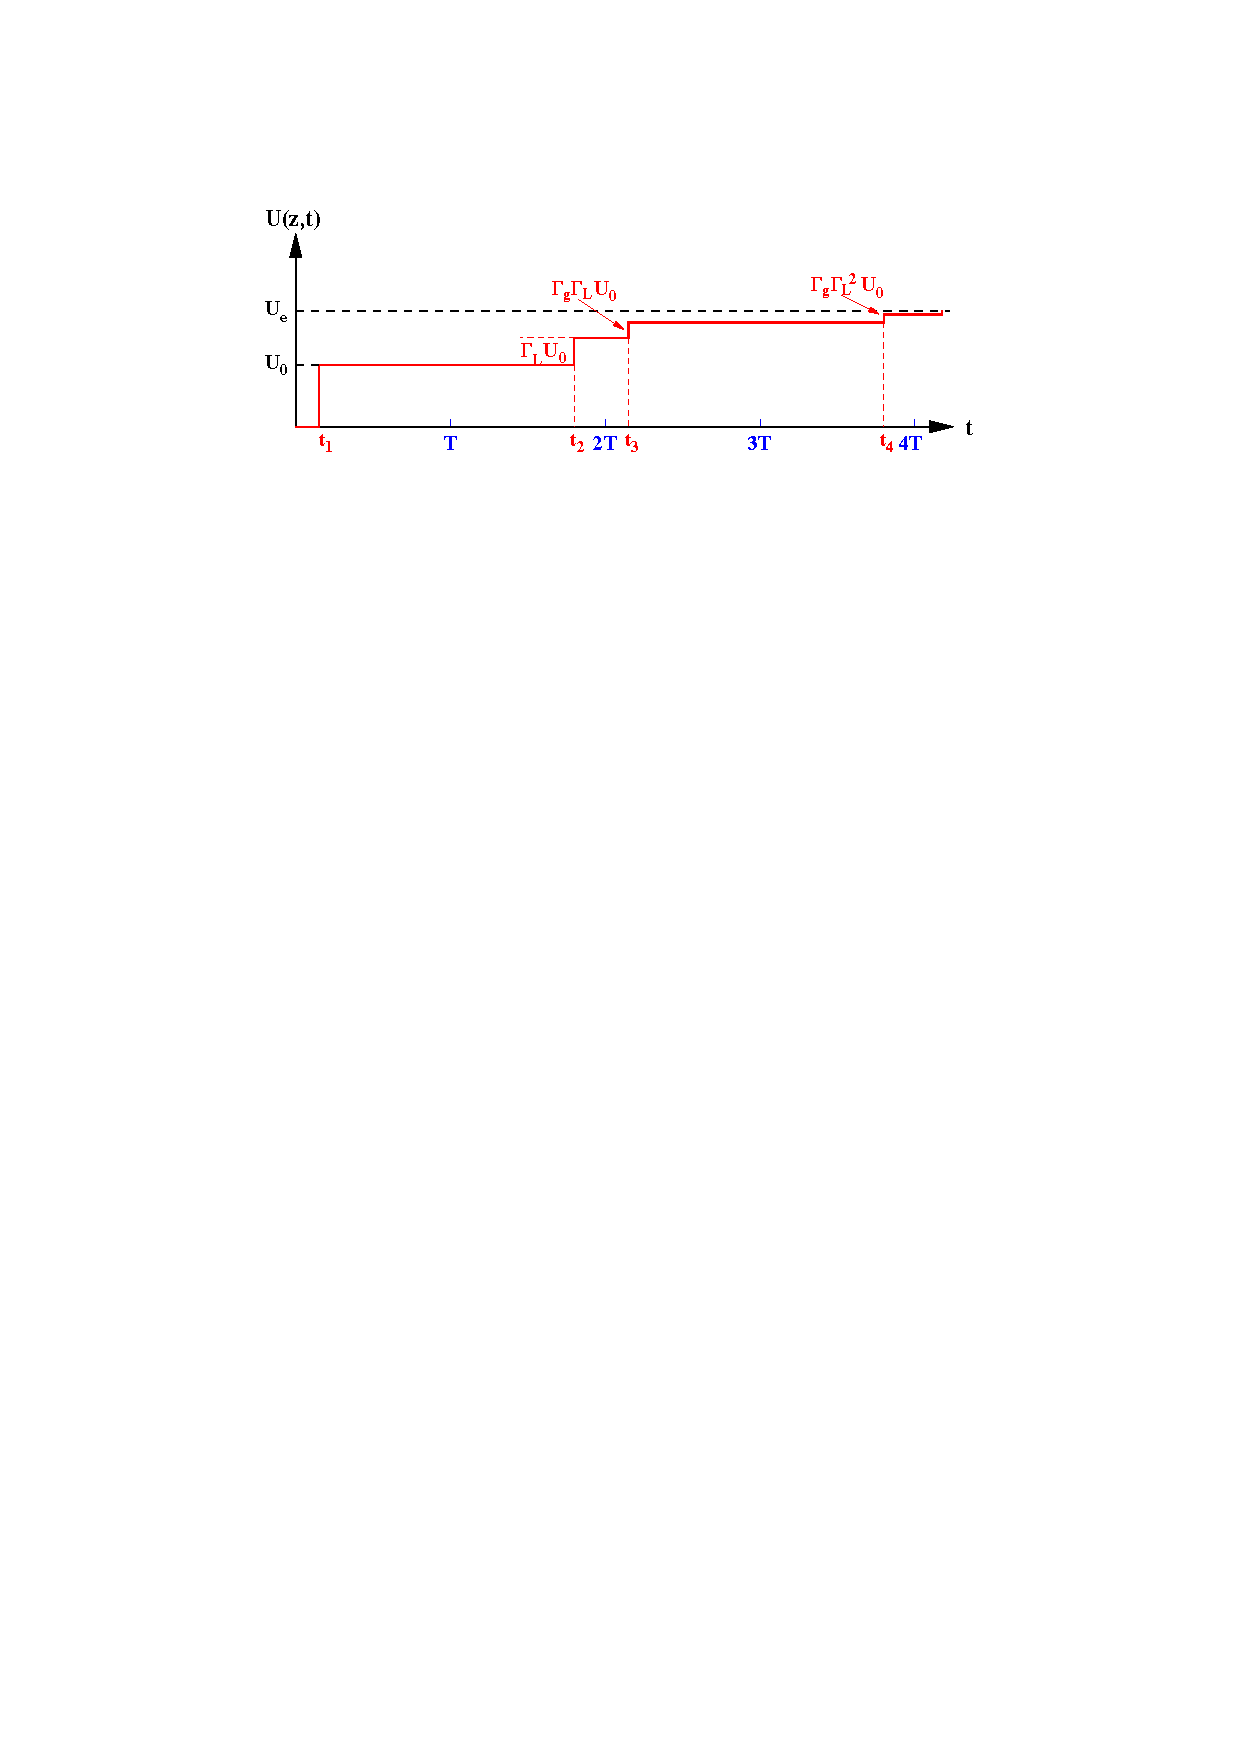
\includegraphics[width=0.9\linewidth]{img/spannung-zeit.pdf}
    \caption{
        Spannungs-Zeit-Verlauf eines Spannungspulses bei Reflexion an einem
        Lastwiderstand [E02].
        In diesem Diagramm sind keine Störstellen enthalten.
    }
    \label{fig:spannung-zeit}
\end{figure}
% subsection impulsfahrplan (end)

\subsection{Koaxialkabel} % (fold)
\label{sub:koaxialkabel}
In diesem Versuch wird als Leiter ein Koaxialkabel herangezogen.
Das Kabel besteht aus einem zylinderförmigen, äußeren Leiter,
der einen inneren Leiter umschließt und von diesem mit einem
Dielektrikum getrennt ist.
Eine besonderheit des Koaxialkabels ist das verschwindende äußere
Feld, weshalb Signalübertragungen über diesen Kabeltyp vergleichsweise
wenig störanfällig sind.
Die Leitungskonstanten, die die Eigenschafen des Kabels beschreiben
sind stark von dessen Innen- und
Ausserndurchmesser $d$ und $D$, beziehungsweise von dem Verhältnis
$\sfrac{D}{d}$ abhängig:
\begin{align*}
    \text{\small Widerstand}\quad R &\propto \left(\frac{1}{d}+\frac{1}{D}\right) &
    \text{\small Induktivität}\quad L &\propto \text{ln}\left(\frac{D}{d}\right) \\
    \text{\small Querleitwert}\quad G &\propto \frac{1}{\text{ln}\left(D/d\right)} &
    \text{\small Kapazität}\quad C &\propto \frac{1}{\text{ln}\left(D/d\right)} \\
\end{align*}
Bei hochfrequenten Wechselströmen im Leiter werden Leiterwiderstand $R$ und
Querleitwert $G$ frequenzabhängig.
Der Widerstand $R$ folgt in diesem Bereich einer $\sqrt{\omega}$-Abhängigkeit
(Skin-Effekt).
% subsection koaxialkabel (end)

\subsection{Impedanzanpassung} % (fold)
\label{sub:impedanzanpassung}
Wie in Abschnitt \ref{sub:signalpulse} erwähnt, ist es für eine effiziente
Signalübertragung wünschenswert, die Leitung an die Impedanz der Last
anzupassen, um den reflektierten Anteil $\Gamma_\text{L}U_0$ der Welle zu
minimieren.
Mit Kenntnis von Abschlussimpedanz $Z_\text{L}$ und Wellenwiderstand $Z_0$
lässt sich hierbei der Reflektionsfaktor $\Gamma$ einer Leitung mit Hilfe
eines Smith-Diagrammes bestimmen.
Dabei werden Real- und Imaginärteil der Normierten Impedanz
$z_\text{L} = Z_\text{L}/Z_0$ möbius-transformiert und als Kreise in der
Impulsebene aufgetragen.
Der Betrag des Reflexionskoeffizienten $\Gamma$ und die Phase $\varphi$ können
dann, wie in Abbildung \ref{fig:smith} dargestellt, abgelesen werden.
\begin{figure}
    \centering
    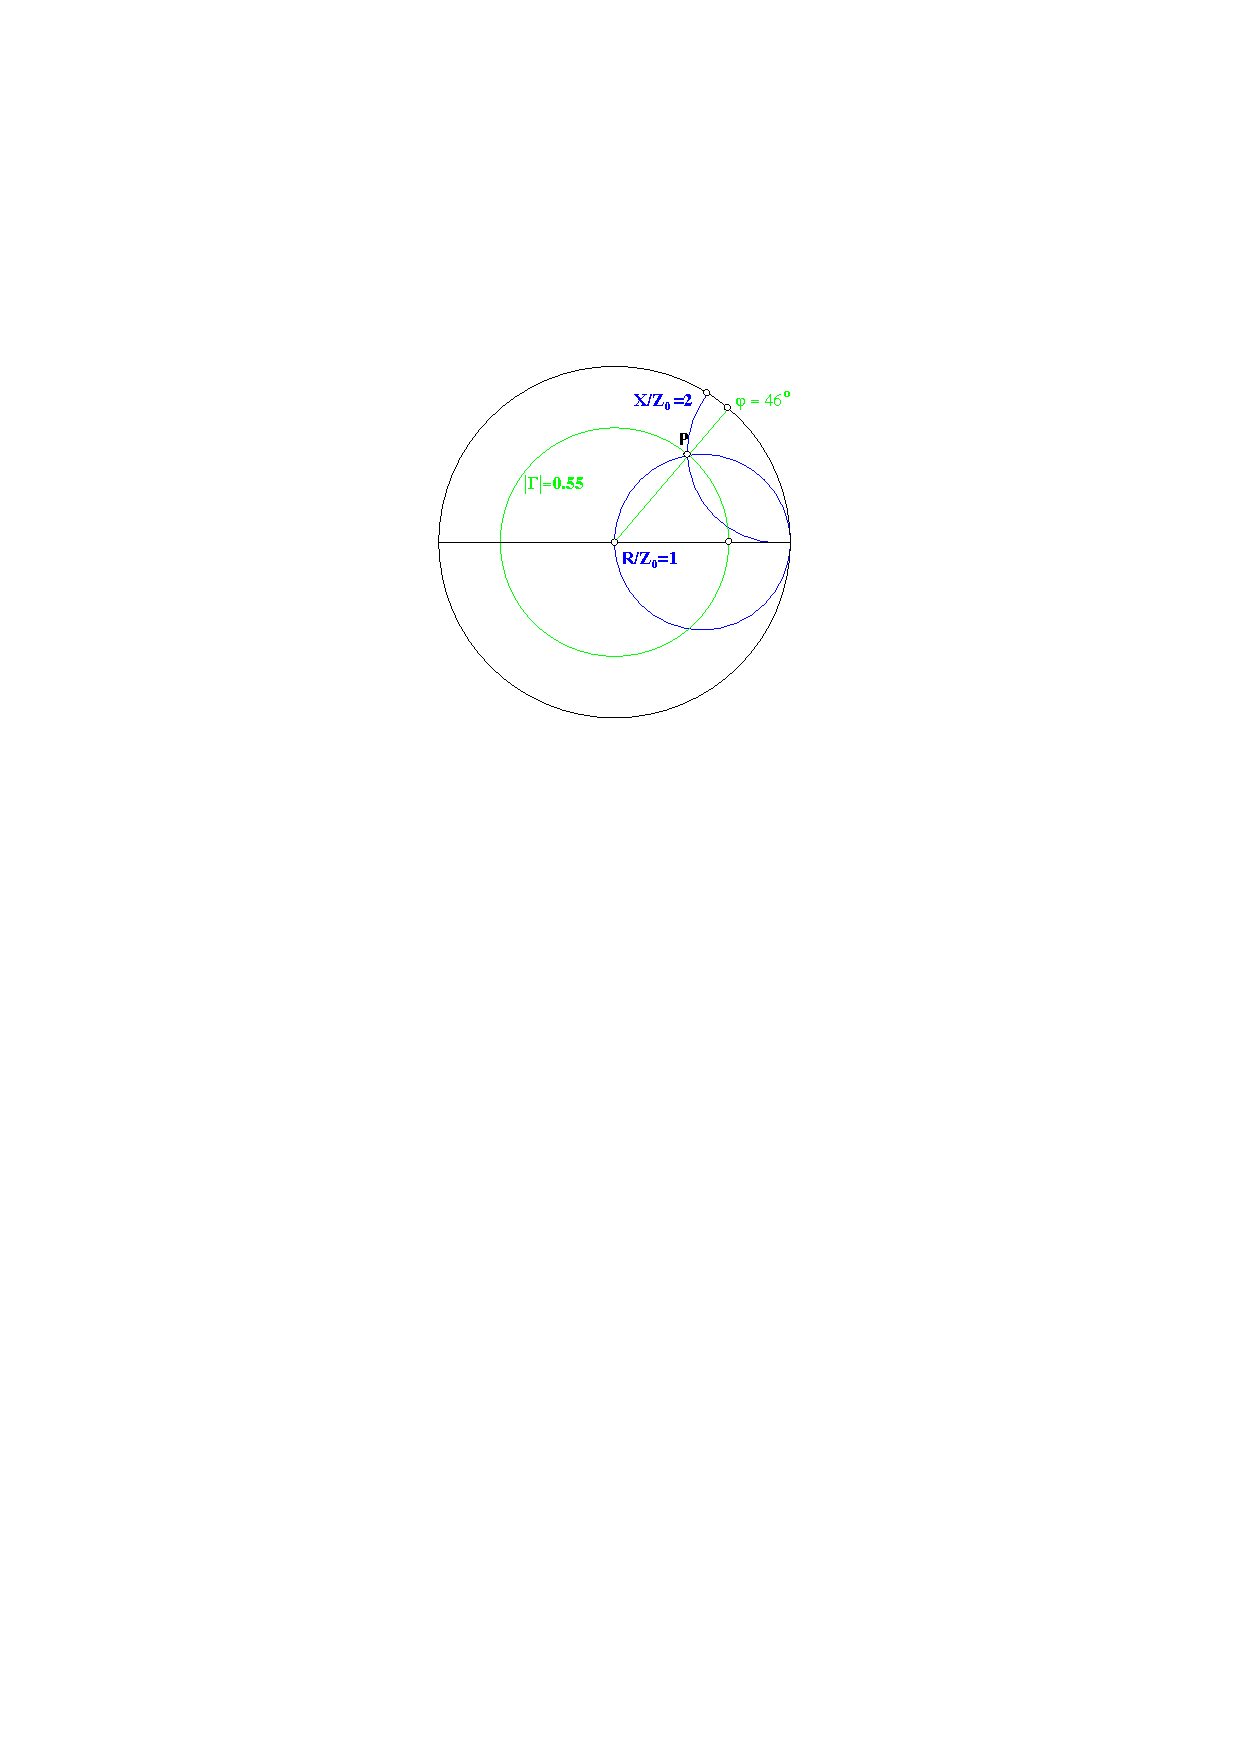
\includegraphics[width=0.7\linewidth]{img/smith.pdf}
    \caption{
        Smith-Diagramm am Beispiel einer normierten Impedanz
        $z_\text{L} = (\num{50}+\num{100}\i)\si{\ohm}/\num{50}\si{\ohm}$
        [E02].
    }
    \label{fig:smith}
\end{figure}
% subsection impedanzanpassung (end)
% section grundlagen (end)
\section{Aufbau} % (fold)
\label{sec:aufbau}
Der Versuchsaufbau umfasst einen Signalgenerator, der Rechteckpulse generiert,
ein Oszilloskop, welches den Signalverlauf zeitaufgelöst messen kann und
verschiedene Abschlüsse und Lasten, und ist in Abbildung \ref{fig:aufbau}
dargestellt.
\begin{figure}
    \centering
    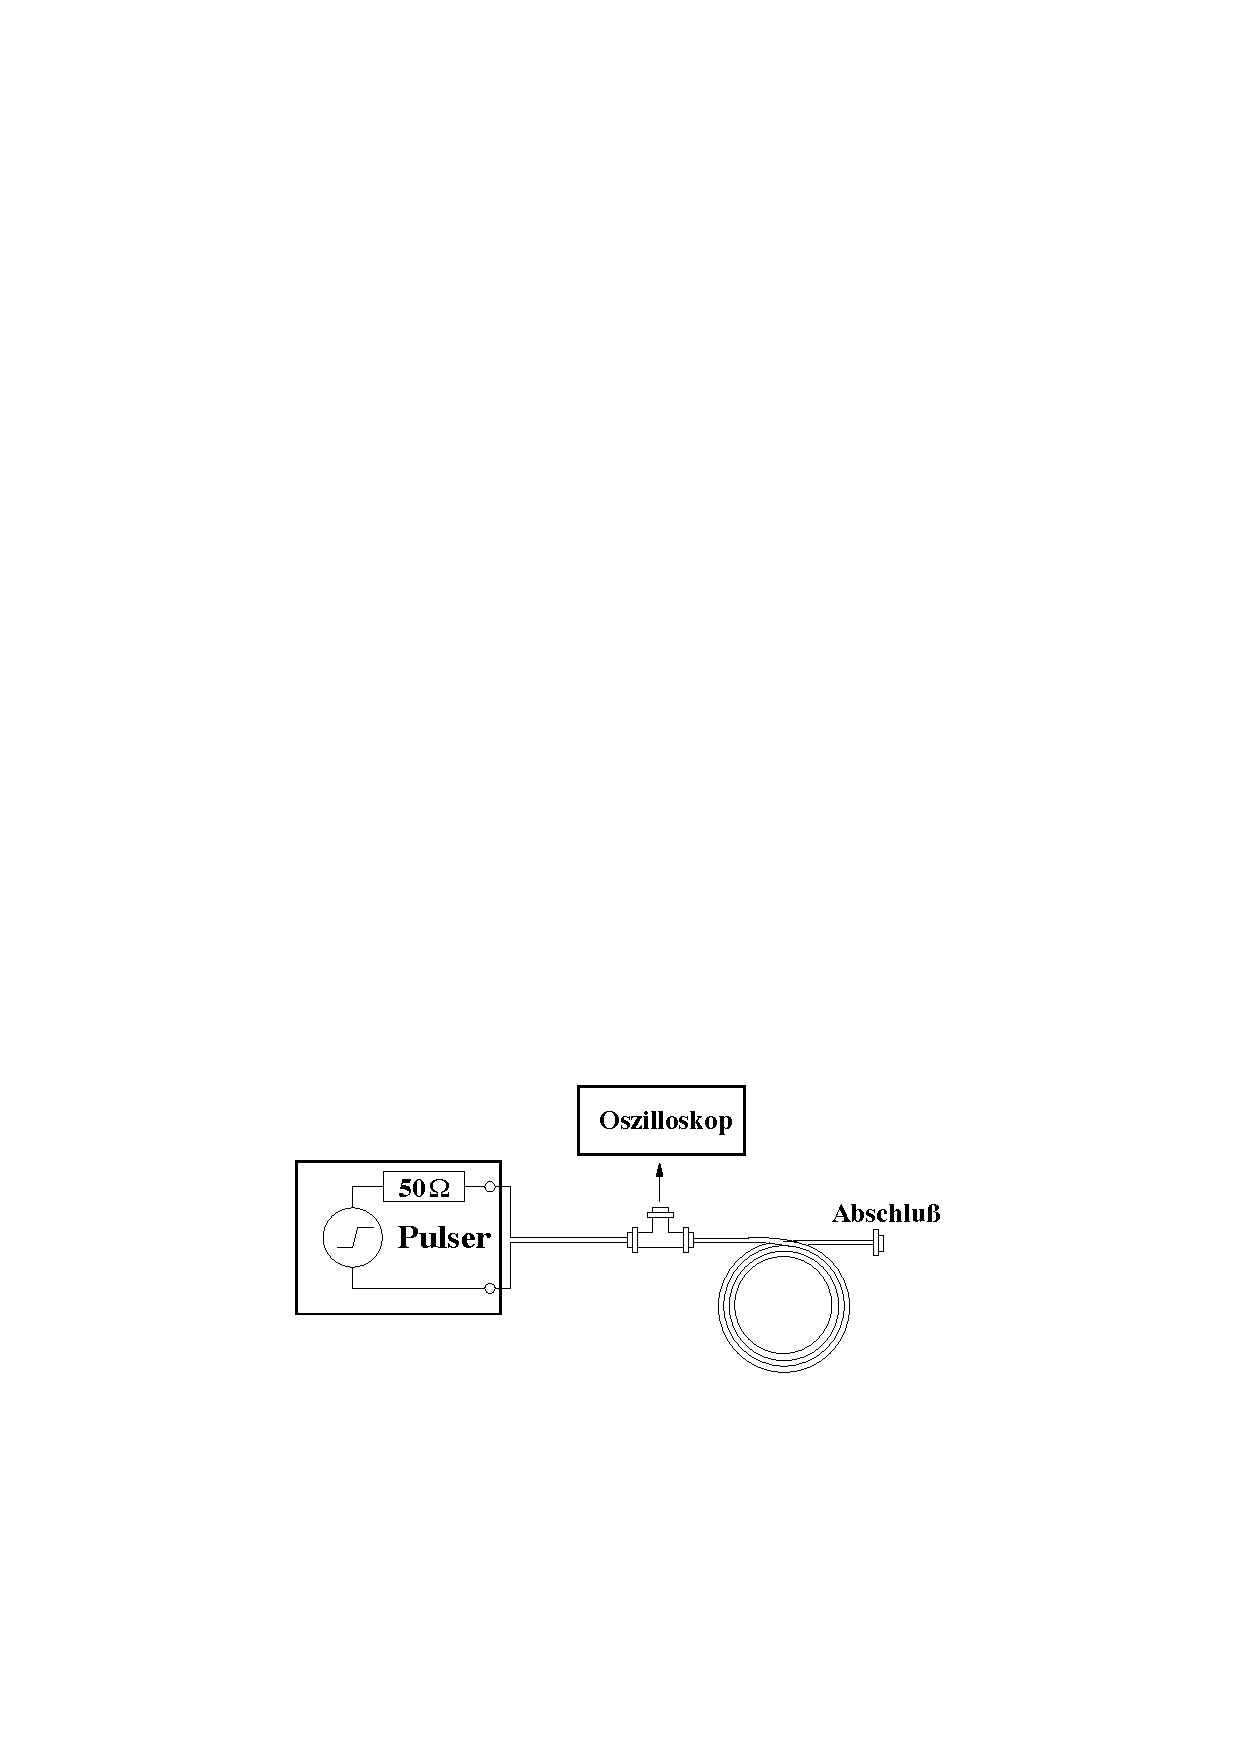
\includegraphics[width=0.7\linewidth]{img/aufbau.pdf}
    \caption{
        Versuchsaufbau für die Untersuchung von Signalen auf Leitungen
        [E02].
    }
    \label{fig:aufbau}
\end{figure}

% section aufbau (end)
